\documentclass[border=5pt]{standalone}
\usepackage{tikz}
\usetikzlibrary{positioning, arrows.meta, fit, backgrounds, calc, shapes.geometric, decorations.pathreplacing}
\usepackage[T1]{fontenc}

\definecolor{backendblue}{HTML}{DAE8FC}
\definecolor{backendstroke}{HTML}{6C8EBF}
\definecolor{simgreen}{HTML}{D5E8D4}
\definecolor{simstroke}{HTML}{82B366}
\definecolor{physpurple}{HTML}{E1D5E7}
\definecolor{physstroke}{HTML}{9673A6}
\definecolor{envorange}{HTML}{FFE6CC}
\definecolor{envstroke}{HTML}{D6B656}
\definecolor{compfill}{HTML}{F5F5F5}
\definecolor{compstroke}{HTML}{666666}

\begin{document}
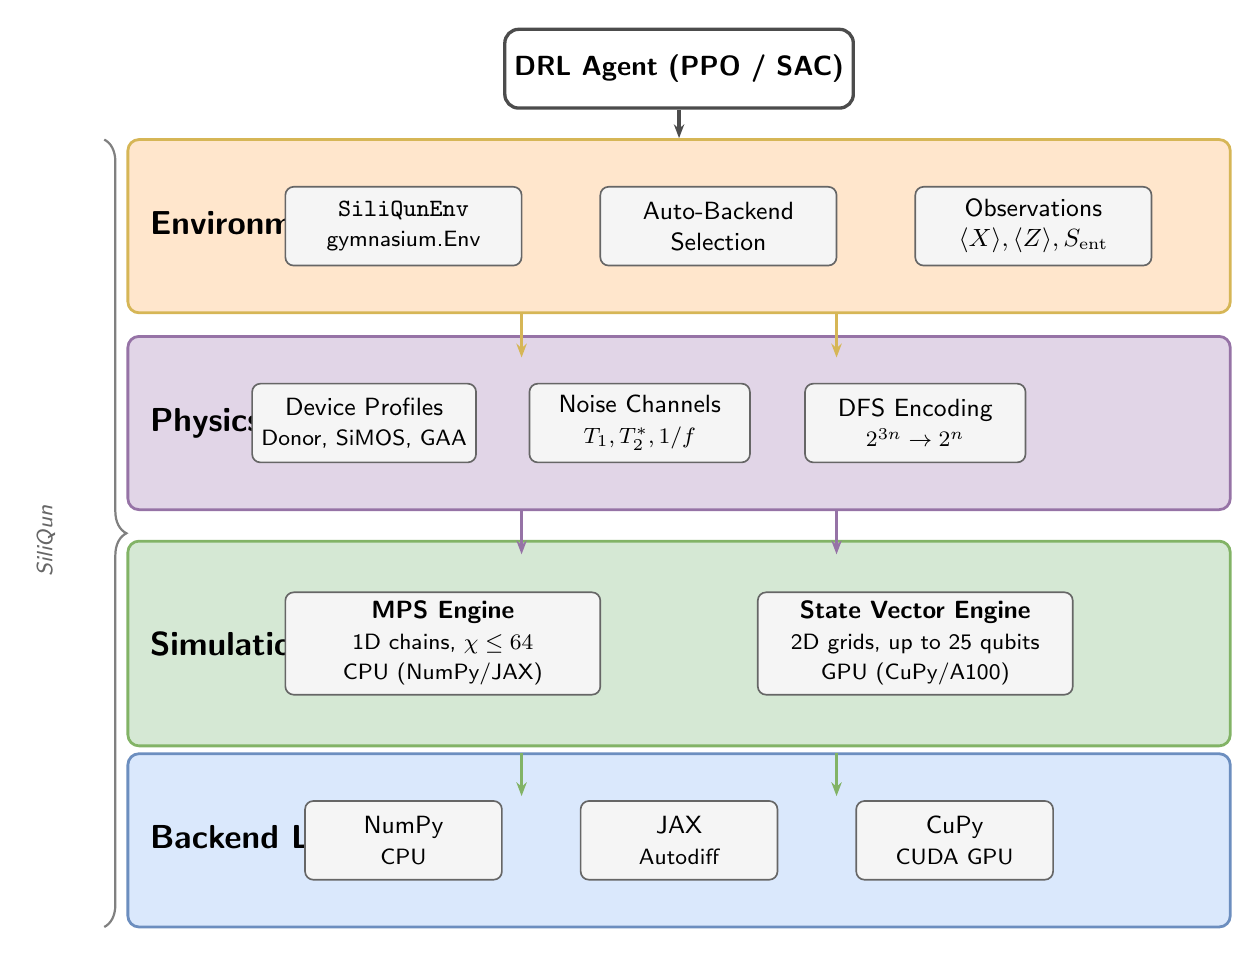
\begin{tikzpicture}[
    layer/.style={
        draw, rounded corners=4pt, minimum width=14cm, minimum height=2.2cm,
        font=\sffamily\bfseries\large, text=black, align=center,
        line width=1pt
    },
    comp/.style={
        draw=compstroke, fill=compfill, rounded corners=3pt,
        minimum width=3.5cm, minimum height=1cm,
        font=\sffamily\small, align=center, line width=0.6pt
    },
    arr/.style={
        -{Stealth[length=5pt]}, line width=1.2pt, color=#1
    },
    larr/.style={
        {Stealth[length=5pt]}-{Stealth[length=5pt]}, line width=1pt, color=#1, dashed
    }
]

% Layer 4: Environment (top)
\node[layer, fill=envorange, draw=envstroke] (env) at (0, 7.5) {};
\node[font=\sffamily\bfseries\large, anchor=west] at ([xshift=5pt]env.west) {Environment Layer};

\node[comp, minimum width=3cm] (gymenv) at (-3.5, 7.5) {\texttt{SiliQunEnv}\\\footnotesize gymnasium.Env};
\node[comp, minimum width=3cm] (autosel) at (0.5, 7.5) {Auto-Backend\\Selection};
\node[comp, minimum width=3cm] (obs) at (4.5, 7.5) {Observations\\$\langle X\rangle, \langle Z\rangle, S_\mathrm{ent}$};

% Layer 3: Physics
\node[layer, fill=physpurple, draw=physstroke] (phys) at (0, 5) {};
\node[font=\sffamily\bfseries\large, anchor=west] at ([xshift=5pt]phys.west) {Physics Layer};

\node[comp, minimum width=2.8cm] (devprof) at (-4, 5) {Device Profiles\\\footnotesize Donor, SiMOS, GAA};
\node[comp, minimum width=2.8cm] (noise) at (-0.5, 5) {Noise Channels\\\footnotesize $T_1, T_2^*, 1/f$};
\node[comp, minimum width=2.8cm] (dfs) at (3, 5) {DFS Encoding\\\footnotesize $2^{3n} \to 2^n$};

% Layer 2: Simulation Core
\node[layer, fill=simgreen, draw=simstroke, minimum height=2.6cm] (sim) at (0, 2.2) {};
\node[font=\sffamily\bfseries\large, anchor=west] at ([xshift=5pt]sim.west) {Simulation Core};

\node[comp, minimum width=4cm, minimum height=1.3cm] (mps) at (-3, 2.2) {\textbf{MPS Engine}\\\footnotesize 1D chains, $\chi \leq 64$\\\footnotesize CPU (NumPy/JAX)};
\node[comp, minimum width=4cm, minimum height=1.3cm] (sv) at (3, 2.2) {\textbf{State Vector Engine}\\\footnotesize 2D grids, up to 25 qubits\\\footnotesize GPU (CuPy/A100)};

% Layer 1: Backend
\node[layer, fill=backendblue, draw=backendstroke] (back) at (0, -0.3) {};
\node[font=\sffamily\bfseries\large, anchor=west] at ([xshift=5pt]back.west) {Backend Layer};

\node[comp, minimum width=2.5cm] (numpy) at (-3.5, -0.3) {NumPy\\\footnotesize CPU};
\node[comp, minimum width=2.5cm] (jax) at (0, -0.3) {JAX\\\footnotesize Autodiff};
\node[comp, minimum width=2.5cm] (cupy) at (3.5, -0.3) {CuPy\\\footnotesize CUDA GPU};

% Vertical arrows between layers
\draw[arr=envstroke] (env.south) +(-2,0) -- +(-2,-0.55);
\draw[arr=envstroke] (env.south) +(2,0) -- +(2,-0.55);
\draw[arr=physstroke] (phys.south) +(-2,0) -- +(-2,-0.55);
\draw[arr=physstroke] (phys.south) +(2,0) -- +(2,-0.55);
\draw[arr=simstroke] ([yshift=-2pt]sim.south) +(-2,0) -- +(-2,-0.55);
\draw[arr=simstroke] ([yshift=-2pt]sim.south) +(2,0) -- +(2,-0.55);

% DRL Agent on top
\node[draw=black!70, fill=white, rounded corners=5pt, minimum width=4cm, minimum height=1cm,
      font=\sffamily\bfseries, line width=1.2pt] (agent) at (0, 9.5) {DRL Agent (PPO / SAC)};
\draw[arr=black!70] (agent.south) -- (env.north);

% Labels on left
\node[font=\sffamily\footnotesize\itshape, text=black!60, rotate=90, anchor=south] at (-7.8, 3.5) {SiliQun};

% Brace on left
\draw[decorate, decoration={brace, amplitude=8pt, mirror}, line width=0.8pt, color=black!50]
    (-7.3, -1.4) -- (-7.3, 8.6);

\end{tikzpicture}
\end{document}
